\documentclass[11pt, a4paper]{article}
\usepackage{pdfpages}
\usepackage{parallel}
\usepackage[T2A]{fontenc}
\usepackage{ucs}
\usepackage[utf8x]{inputenc}
\usepackage[polish,english,russian]{babel}
\usepackage{hyperref}
\usepackage{rotating}
\usepackage[inner=2cm,top=1.8cm,outer=2cm,bottom=2.3cm,nohead]{geometry}
\usepackage{listings}
\usepackage{graphicx}
\usepackage{wrapfig}
\usepackage{longtable}
\usepackage{indentfirst}
\usepackage{array}
\usepackage{tikzsymbols}
\usepackage{soul}
\usepackage[ruled,vlined]{algorithm2e}
%\counterwithout{figure}{section} 

\usepackage{url}
\makeatletter
\g@addto@macro{\UrlBreaks}{\UrlOrds}
\makeatother

\newcolumntype{P}[1]{>{\raggedright\arraybackslash}p{#1}}
\frenchspacing
\usepackage{fixltx2e} %text sub- and superscripts
\usepackage{icomma} % коскі ў матэматычным рэжыме
\PreloadUnicodePage{4}

\newcommand{\longpage}{\enlargethispage{\baselineskip}}
\newcommand{\shortpage}{\enlargethispage{-\baselineskip}}

\def\switchlang#1{\expandafter\csname switchlang#1\endcsname}
\def\switchlangbe{
\let\saverefname=\refname%
\def\refname{Літаратура}%
\def\figurename{Іл.}%
}
\def\switchlangen{
\let\saverefname=\refname%
\def\refname{References}%
\def\figurename{Fig.}%
}
\def\switchlangru{
\let\saverefname=\refname%
\let\savefigurename=\figurename%
\def\refname{Литература}%
\def\figurename{Рис.}%
}

\hyphenation{admi-ni-stra-tive}
\hyphenation{ex-pe-ri-ence}
\hyphenation{fle-xi-bi-li-ty}
\hyphenation{Py-thon}
\hyphenation{ma-the-ma-ti-cal}
\hyphenation{re-ported}
\hyphenation{imp-le-menta-tions}
\hyphenation{pro-vides}
\hyphenation{en-gi-neering}
\hyphenation{com-pa-ti-bi-li-ty}
\hyphenation{im-pos-sible}
\hyphenation{desk-top}
\hyphenation{elec-tro-nic}
\hyphenation{com-pa-ny}
\hyphenation{de-ve-lop-ment}
\hyphenation{de-ve-loping}
\hyphenation{de-ve-lop}
\hyphenation{da-ta-ba-se}
\hyphenation{plat-forms}
\hyphenation{or-ga-ni-za-tion}
\hyphenation{pro-gramming}
\hyphenation{in-stru-ments}
\hyphenation{Li-nux}
\hyphenation{sour-ce}
\hyphenation{en-vi-ron-ment}
\hyphenation{Te-le-pathy}
\hyphenation{Li-nux-ov-ka}
\hyphenation{Open-BSD}
\hyphenation{Free-BSD}
\hyphenation{men-ti-on-ed}
\hyphenation{app-li-ca-tion}

\def\progref!#1!{\texttt{#1}}
\renewcommand{\arraystretch}{2} %Іначай формулы ў матрыцы зліпаюцца з лініямі
\usepackage{array}

\def\interview #1 (#2), #3, #4, #5\par{

\section[#1, #3, #4]{#1 -- #3, #4}
\def\qname{LVEE}
\def\aname{#1}
\def\q ##1\par{{\noindent \bf \qname: ##1 }\par}
\def\a{{\noindent \bf \aname: } \def\qname{L}\def\aname{#2}}
}

\def\interview* #1 (#2), #3, #4, #5\par{

\section*{#1\\{\small\rm #3, #4. #5}}
\ifx\ParallelWhichBox\undefined%
    \addcontentsline{toc}{section}{#1, #3, #4}%
\else%
\ifnum\ParallelWhichBox=0%
    \addcontentsline{toc}{section}{#1, #3, #4}%
\fi\fi%

\def\qname{LVEE}
\def\aname{#1}
\def\q ##1\par{{\noindent \bf \qname: ##1 }\par}
\def\a{{\noindent \bf \aname: } \def\qname{L}\def\aname{#2}}
}

\newcommand{\interviewfooter}[1]{
\vskip 1em
\noindent \textit{#1}
}

\switchlang{en}
\begin{document}

\title{1983 "--- Sharp MZ-1X10 Mouse}
\date{}
\maketitle
\selectlanguage{english}

Sharp MZ-1X10 mouse, known to be the the first mouse in  Japan, practically at the same time when the Microsoft's first mouse, known as the ``green-eyed mouse'' because of its two green buttons. The real manufacturer of both mice was the Japanese company Alps. The MZ-1x10 mouse was intended for use with Sharp MZ-5500 computers, which were based on the Intel 8086 processor, running MS-DOS and aimed at business users \cite{review, wiki}.

\begin{figure}[h]
   \centering
    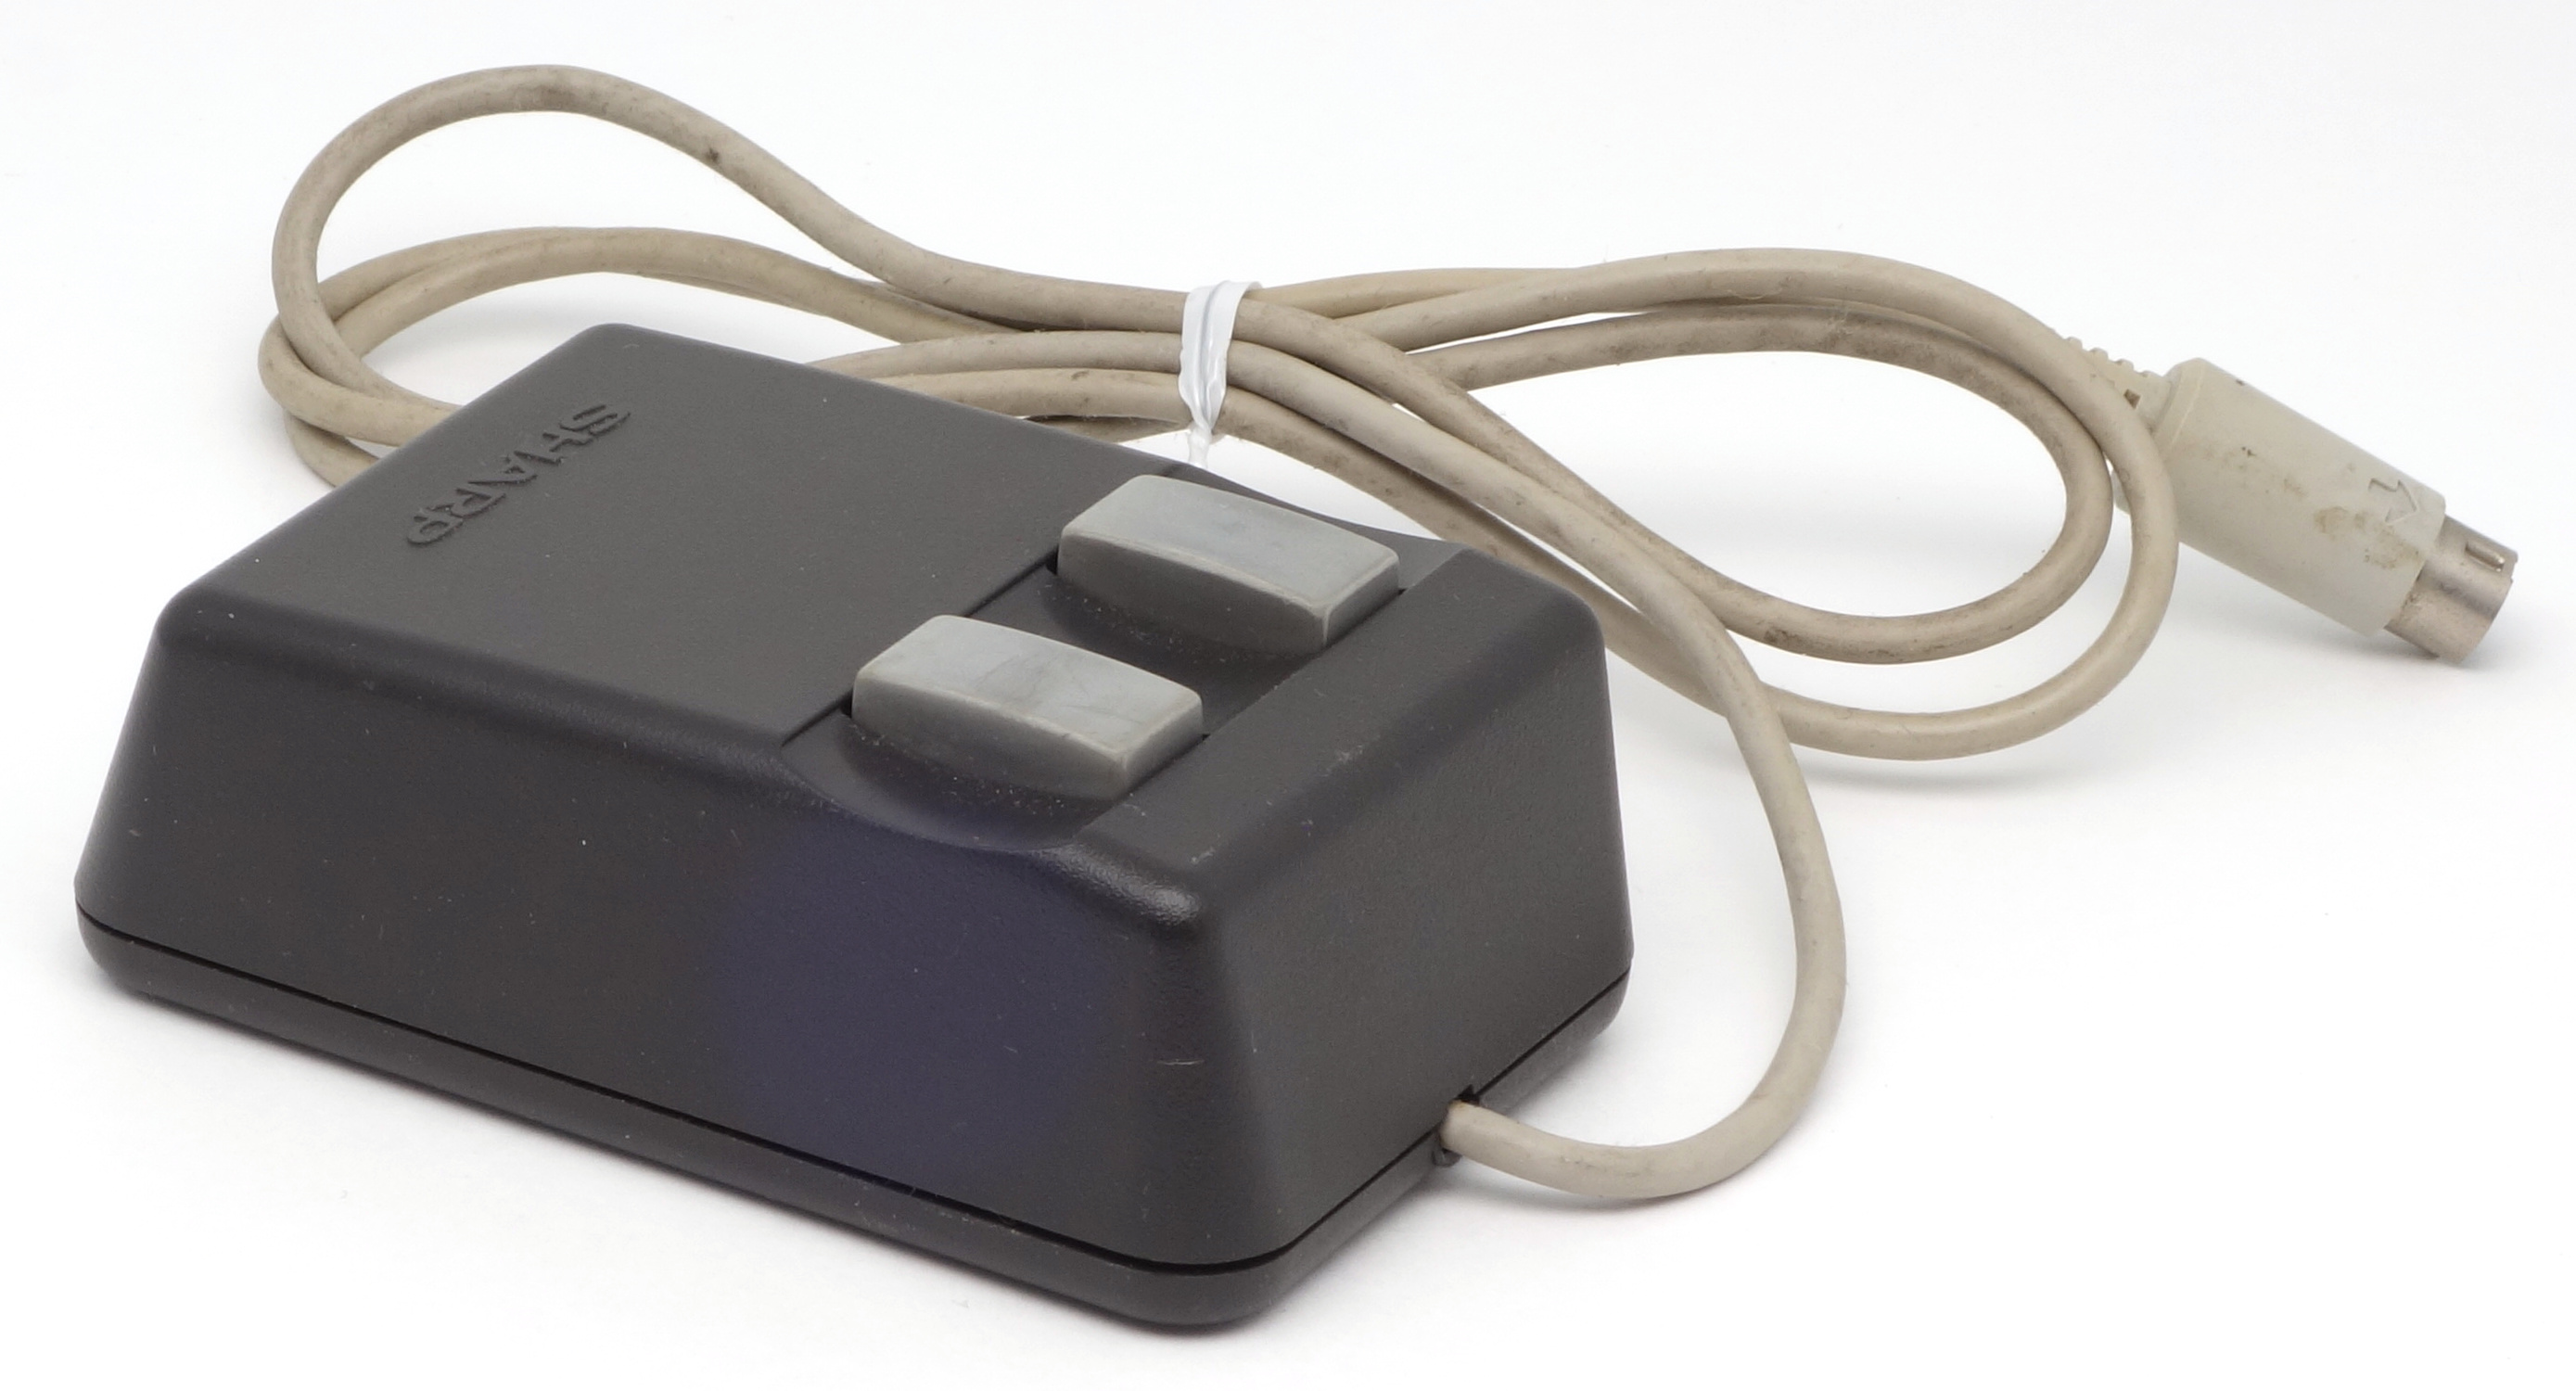
\includegraphics[scale=0.7]{1983_sharp_mz_1x10_mouse/pic_30.jpg}
    \caption{Sharp MZ-1X10 Mouse}
    \label{fig:SharpMZ1x10Pic}
\end{figure}

The body of the MZ-1X10 mouse is a cuboid with slightly rounded edges and a pair of rectangular buttons on the upper side (fig. \ref{fig:SharpMZ1x10Pic}).

\begin{figure}[h]
    \centering
    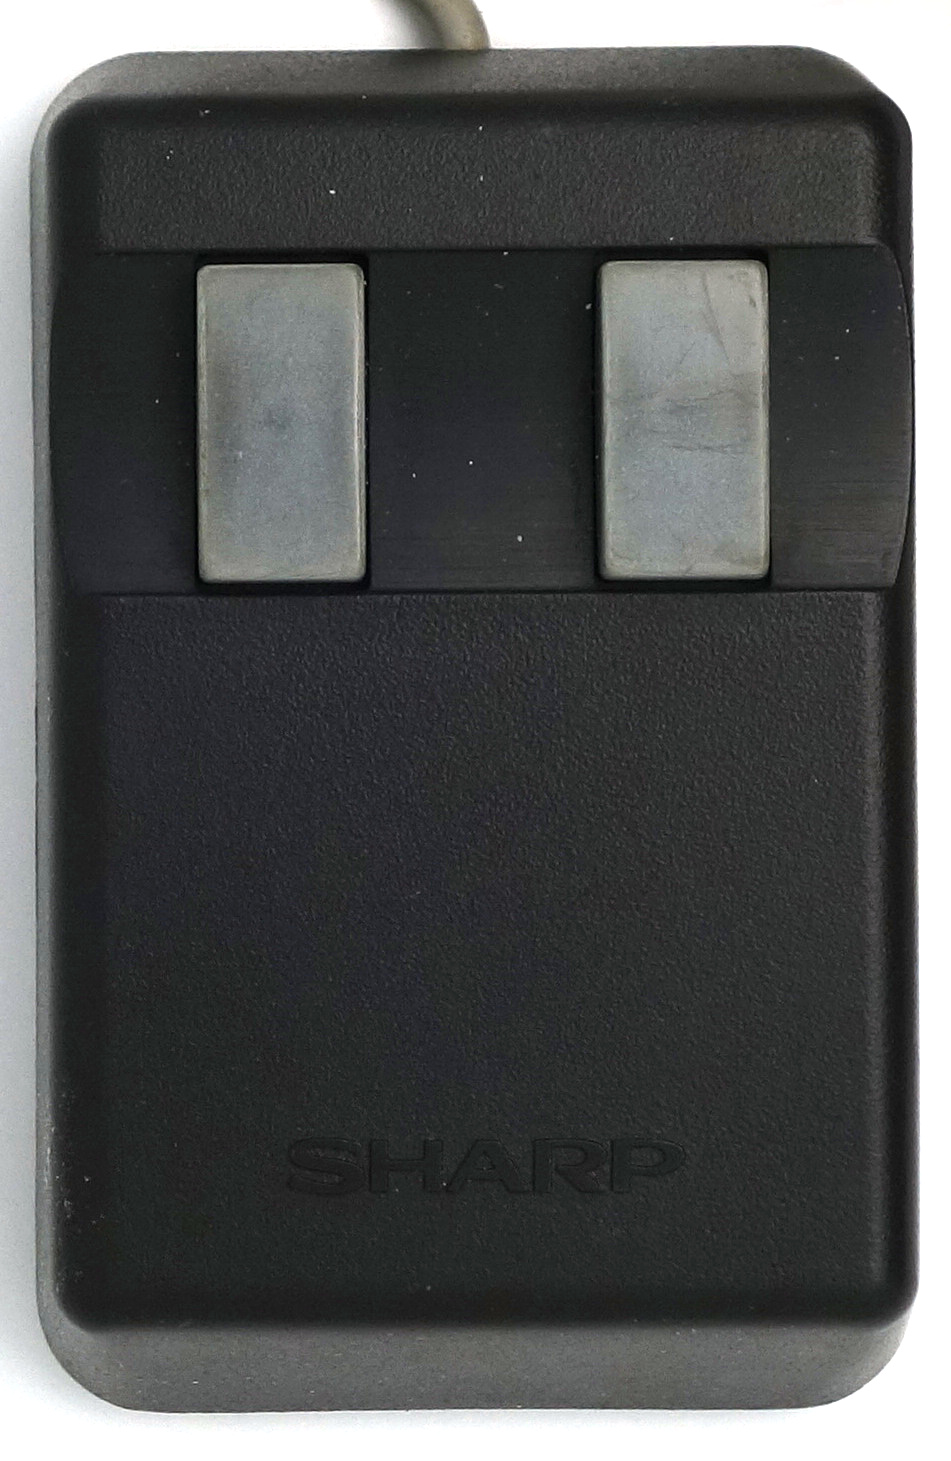
\includegraphics[scale=0.55]{1983_sharp_mz_1x10_mouse/top_15.jpg}
    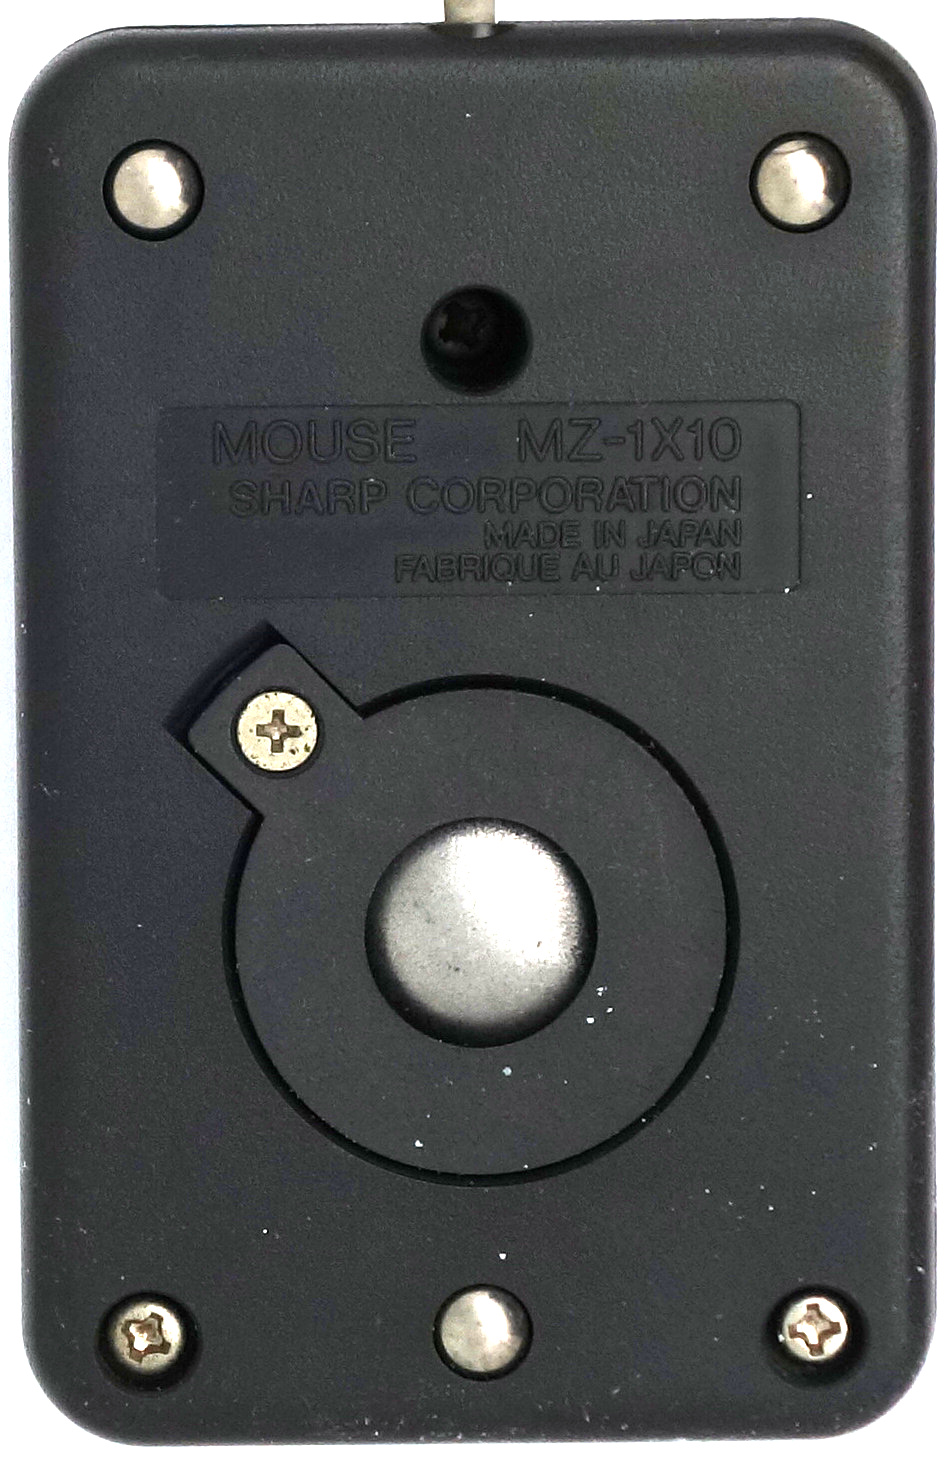
\includegraphics[scale=0.55]{1983_sharp_mz_1x10_mouse/bottom_15.jpg}
    \caption{Sharp MZ-1X10 Mouse, top and bottom views}
    \label{fig:SharpMZ1x10TopAndBottom}
\end{figure}

The bottom side shows steel ball, three small metal balls used as the mouse feet for easier sliding, and a removable ring which would allow removing the ball for cleaning. The latch ring option has not yet been invented, so it must be unscrewed with a screwdriver. The cable has no plastic insert that would protect it from damage in place where it exits the mouse body (fig. \ref{fig:SharpMZ1x10TopAndBottom}).

\begin{figure}[h]
    \centering
    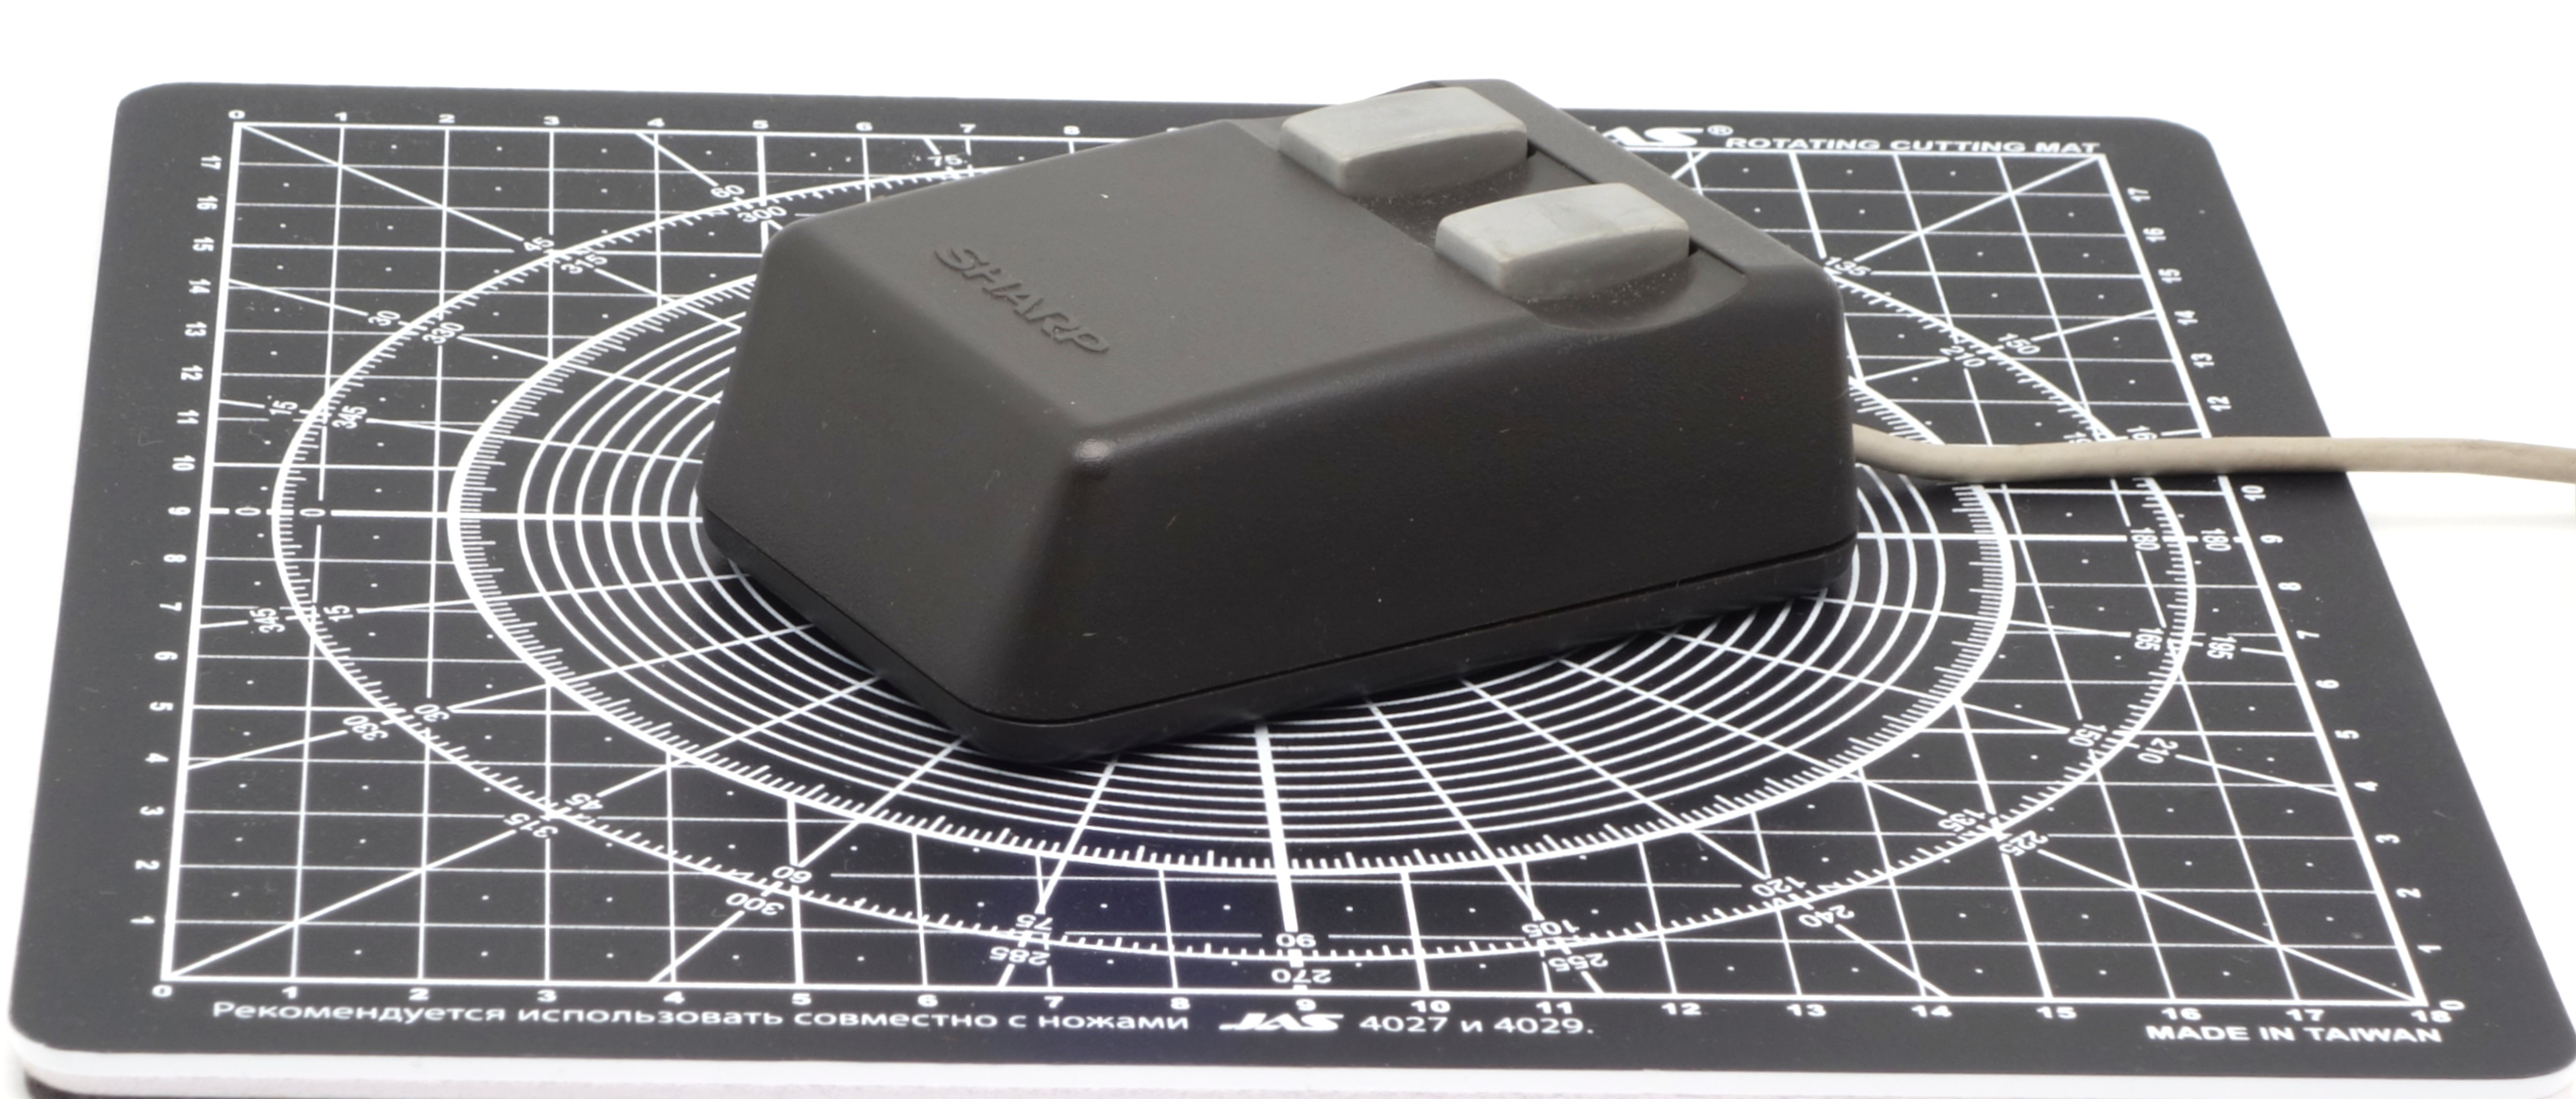
\includegraphics[scale=0.5]{1983_sharp_mz_1x10_mouse/size_30.jpg}
    \caption{Sharp MZ-1X10 Mouse on a graduated pad with a grid step of 1~cm}
    \label{fig:SharpMZ1x10Size}
\end{figure}

Despite the small size of the mouse (fig. \ref{fig:SharpMZ1x10Size}), it is quite heavy. It has a fairly simple design; the shape resembles power supply of a player or some other home gadget of the corresponding time period (or, thanks to specific buttons, automatic fuse for power supply networks). Obviously, the beveled back edge should provide a more comfortable palm position, but taking into account the size this does not bring significant improvements to ergonomics (fig. \ref{fig:SharpMZ1x10Hand}).The buttons are medium in size, acceptable from the comfort point of view.

\begin{figure}[h]
    \centering
    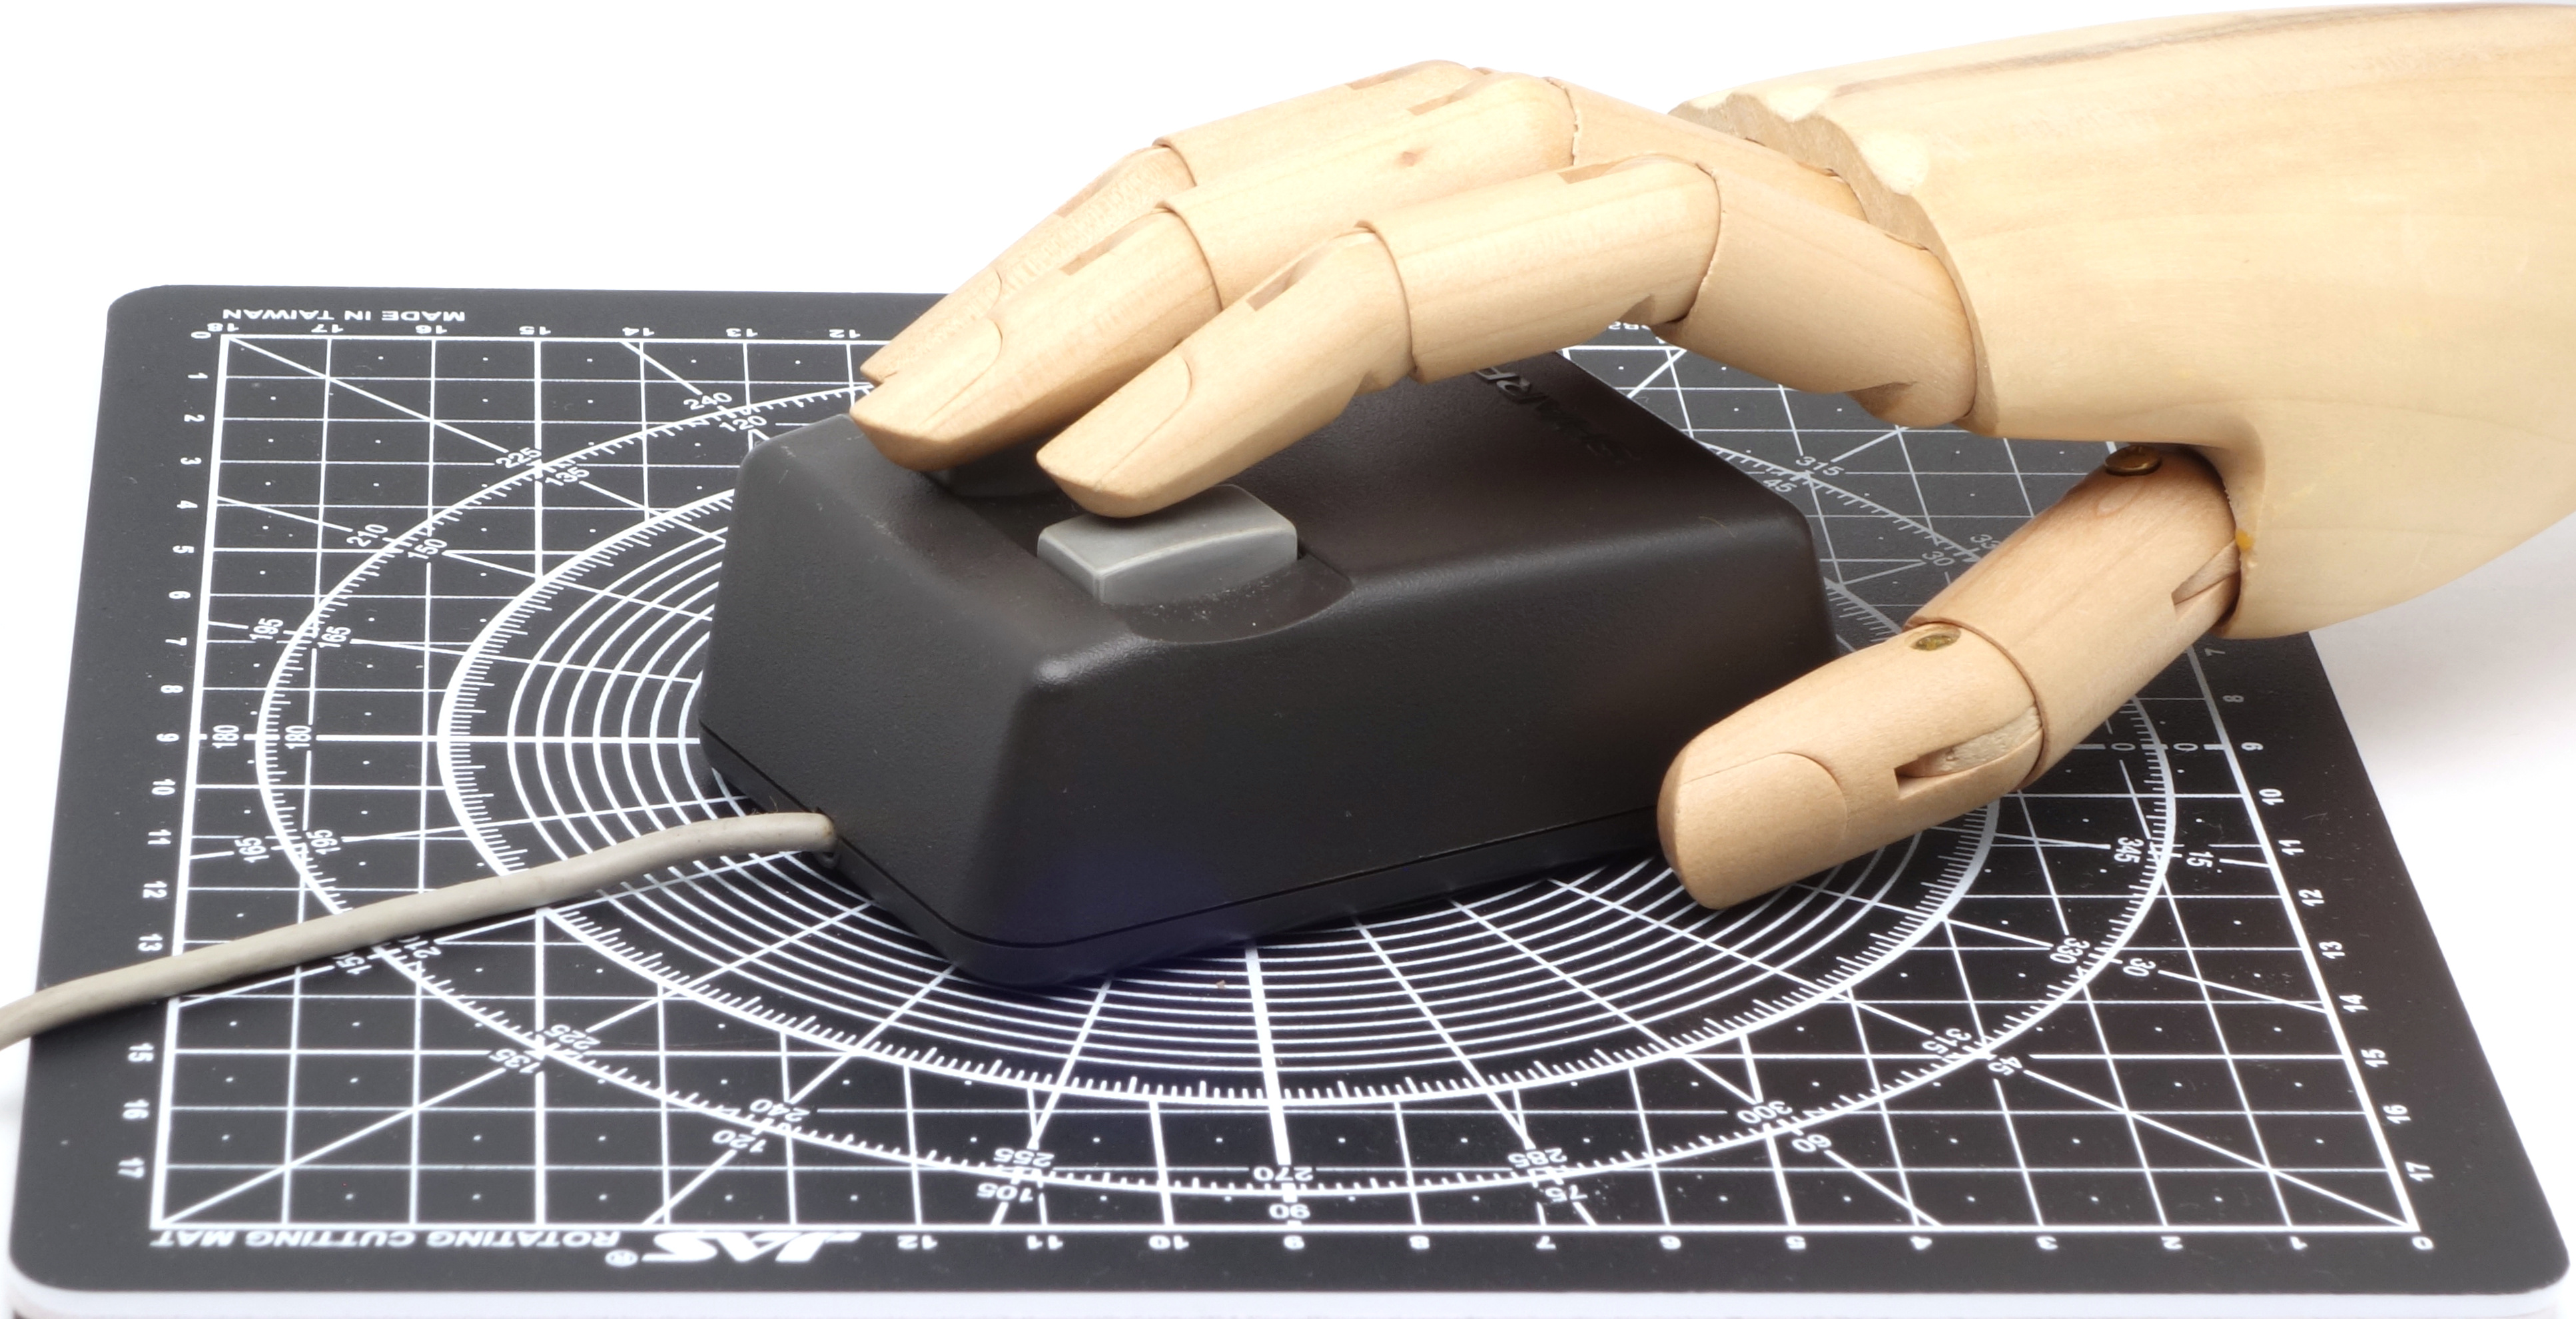
\includegraphics[scale=0.5]{1983_sharp_mz_1x10_mouse/hand_30.jpg}
    \caption{Sharp MZ-1X10 Mouse with a human hand model}
    \label{fig:SharpMZ1x10Hand}
\end{figure}

The mouse was connected to the computer via a serial-type interface. The left button was used to return to the origin (upper left corner of the screen), while the right button worked as the main mouse button, that is, it generated a click in the coordinates corresponding to the cursor position \cite{manual}.

\begin{figure}[h]
    \centering
    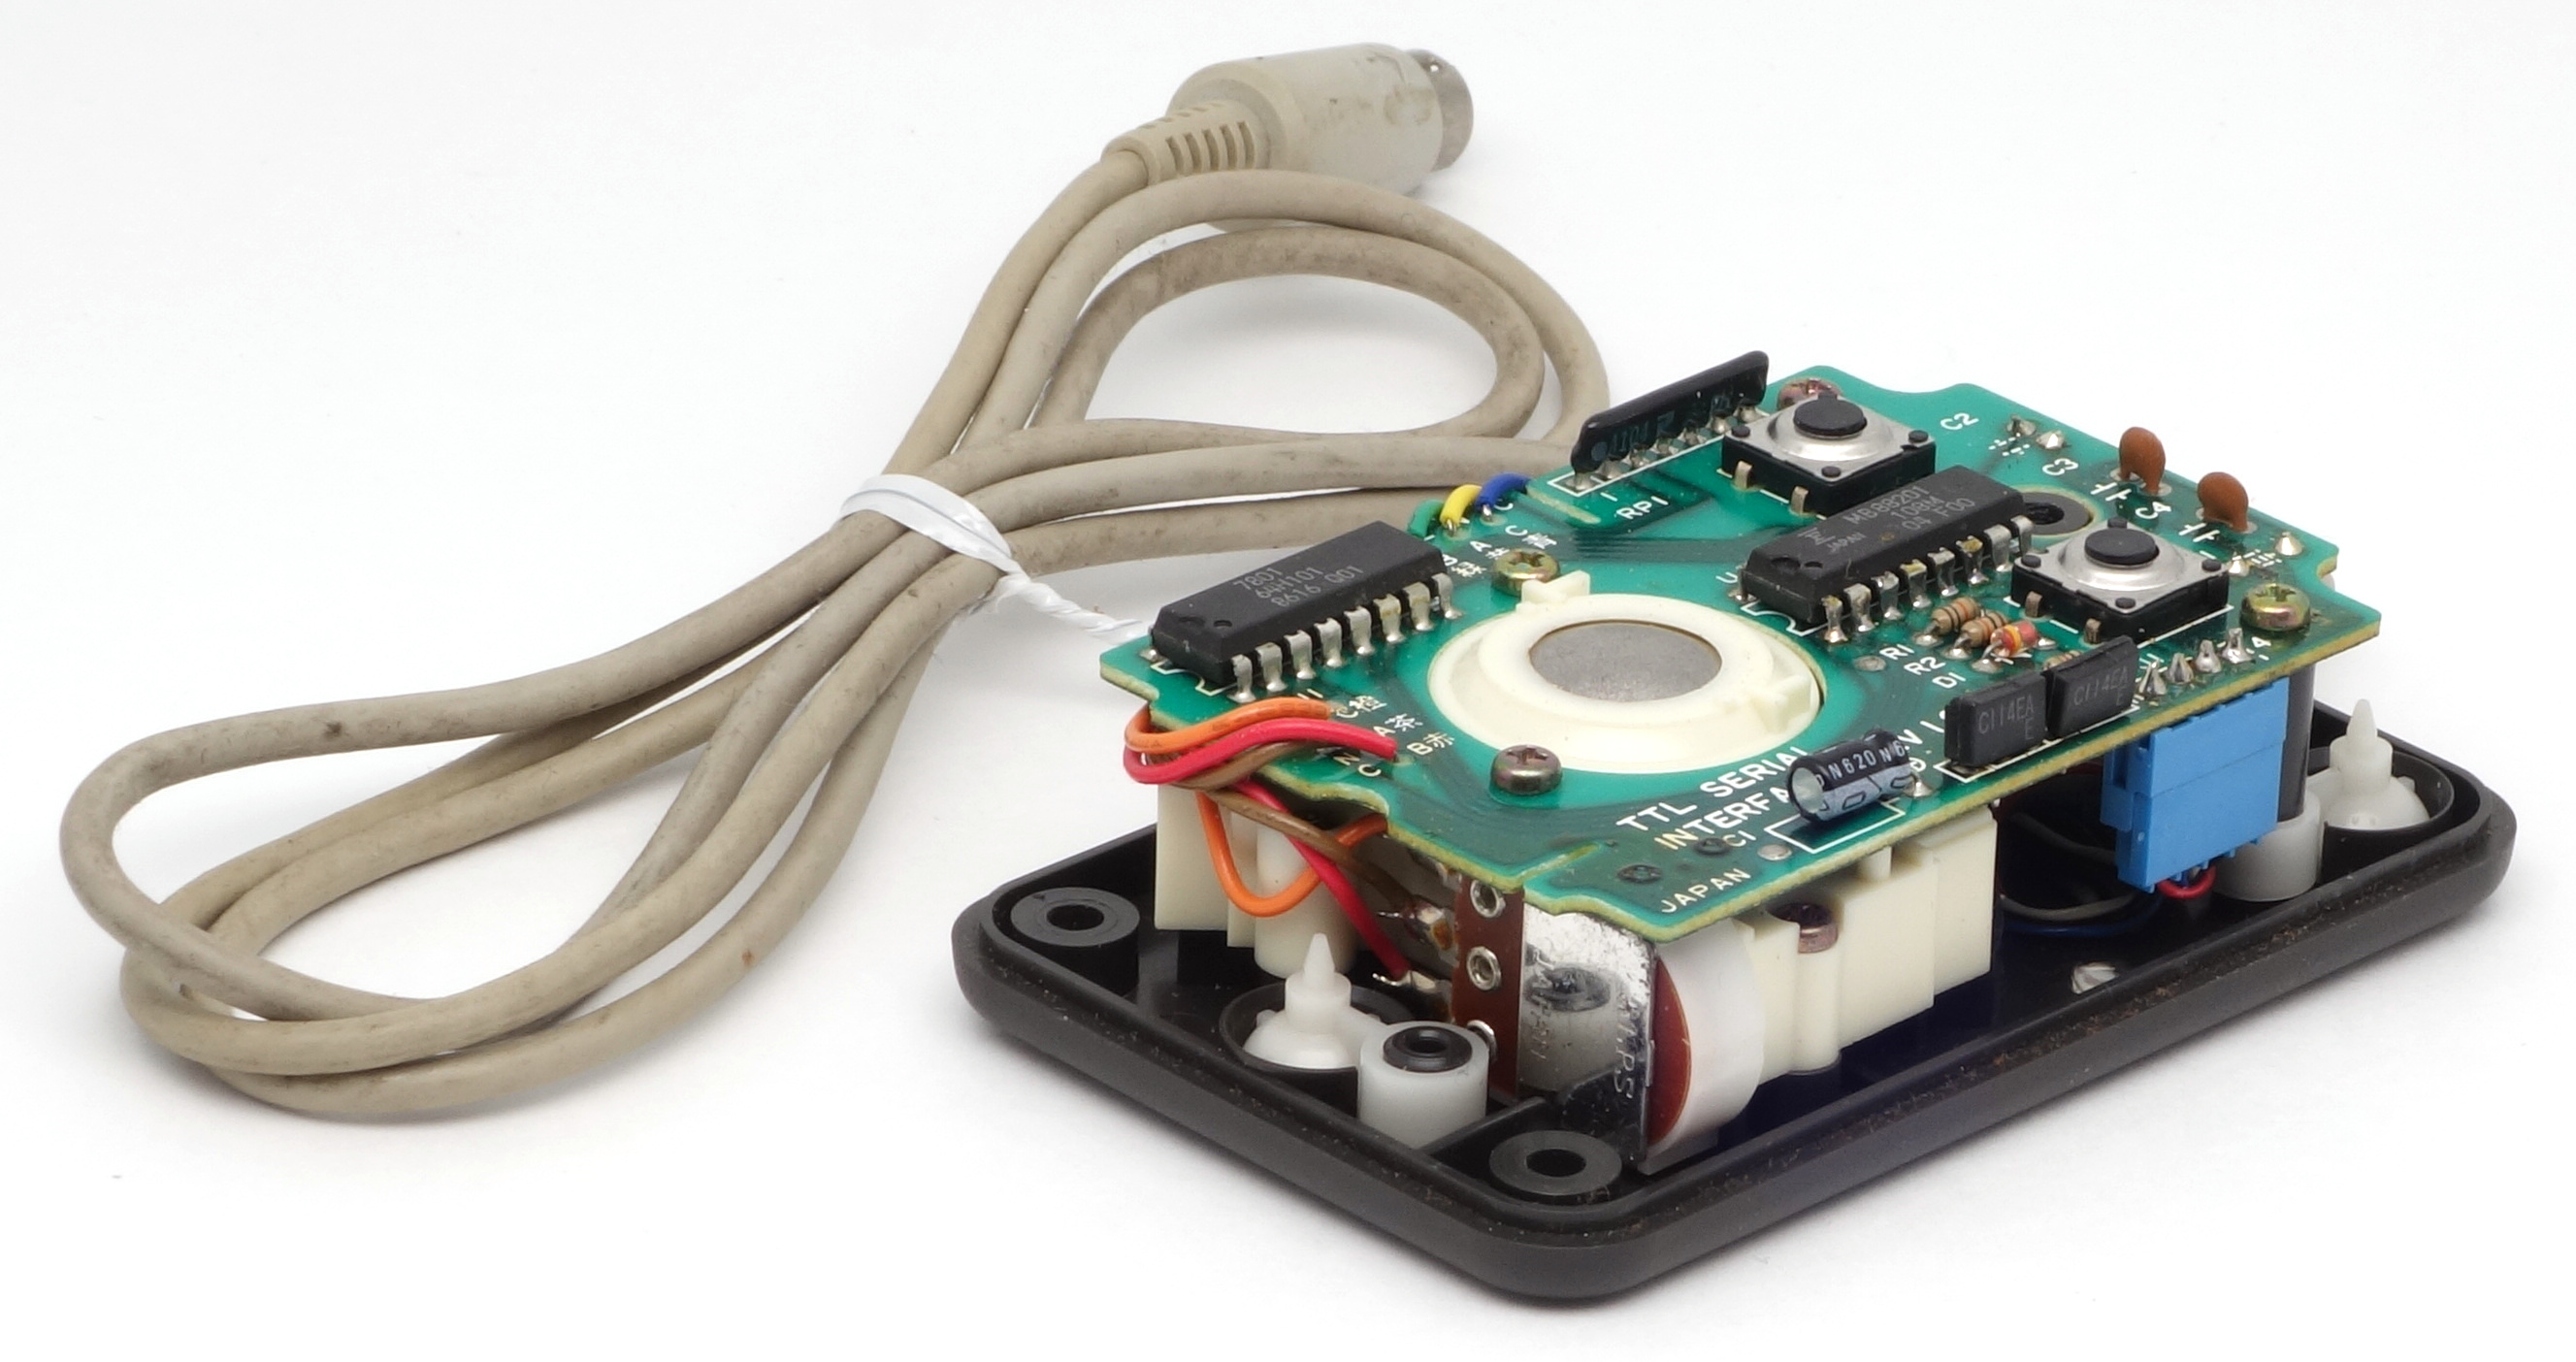
\includegraphics[scale=0.8]{1983_sharp_mz_1x10_mouse/inside_30.jpg}
    \caption{Sharp MZ-1X10 Mouse disassembled}
    \label{fig:SharpMZ1x10Inside}
\end{figure}

The internal structure of the mouse can be seen in fig. \ref{fig:SharpMZ1x10Inside}. The mouse uses closed contact encoders. When compared with the Microsoft green-eyed mouse, the technical design is almost identical: the differences come down to the configuration of the printed circuit board and are obviously caused by the top placement of the buttons.

\begin{thebibliography}{9}
\bibitem{review}  Ohishi Nobuaki. MZ-1X10 (mouse) [in Japanese] \url{http://retropc.net/ohishi/museum/mz1x10.htm}
\bibitem{wiki} Sharp MZ -- Wikipedia \url{https://en.wikipedia.org/wiki/Sharp_MZ#MZ-3500/5500/6500_group}
\bibitem{manual} Sharp MZ-1X10 Instruction Manual \url{https://www.manualslib.com/download/900861/Sharp-Mz-1x10.html}
\end{thebibliography}
\end{document}
